\section{Experiments}
We evaluate the \method{} paradigm across a diverse suite of challenging environments, testing its effectiveness, and demonstrating the scaling law, transferability of the learned experience library, and a thorough case study in all settings.

\subsection{Experimental Setup}
Our experimental setup are structured to comprehensively evaluate the performance and generalizability of \method{}, involving diverse benchmarks, comparisons against established baselines, and a detailed illustration of the training procedures.

\paragraph{Evaluation Benchmarks.}
We evaluate the proposed \method{} paradigm across four challenging benchmarks spanning three scientific domains (\textit{i.e.}, mathematics, chemistry, and biology) to assess both reasoning capability and domain adaptability. Specifically: (1) AIME25 competition dataset~\cite{aime2025problems} for complicated mathematical reasoning; (2) GSM8k dataset~\cite{cobbe2021gsm8k} multi-step arithmetic reasoning; (3) USPTO50k~\cite{schneider2016s} benchmark for canonical single-step retrosynthesis; (4) ProteinGym~\cite{notin2023proteingym} benchmark for protein fitness prediction. 
%These benchmarks collectively cover symbolic, textual, and structured reasoning tasks. 

\paragraph{Compared Methods.}
Our evaluation spans a range of base models, tested on four distinct experimental configurations for comparison: (1) Vanilla LLM, (2) LLM with In-Context Learning (ICL)~\cite{dong2022survey}, (3) LLM agent with reasoning-and-acting workflow (Agent)~\cite{yao2023reactsynergizingreasoningacting}, and (4) our proposed \method{}. For \method{}, each model constructs an experience library during training, which is later utilized at test-time. The library structure is adapted to the benchmark: hierarchical  for AIME25 and USPTO50k, and non-hierarchical for GSM8k and ProteinGym.

\paragraph{Training Configurations.}%Implementation details [这里好像没有涉及implementation？都是在讲trianing/test set如何构建的]
For AIME25, the training was conducted on 49 historical problems from AIME83 to AIME24. On GSM8k, we adhere to the official training and testing splits~\cite{cobbe2021gsm8k}. For USPTO50k, 100 instances are randomly sampled from the original 5k test split for evaluation, and 50 instances from the training split are randomly sampled for training. For ProteinGym, 100 mutational sequences are sampled for each wild-type protein target as training set, which is on average 1.47\% of the available data. This design reflects practical constraints in protein engineering, where only a limited number of labeled mutations are known, while the vast majority of sequence space remains unexplored. %Further details on the experimental protocol are provided in Appendix \xinyuan{To be filled}.

\subsection{Main Results}
Our main results demonstrate that \method{} achieves significant and consistent improvements across all scientific domains and benchmarks, as detailed below.

% Main Results

% Main Table [一般要置顶]
\begin{table}[!t]
\centering
\caption{Results on four benchmarks. All values are accuracies in percentage, which is accuracy for AIME25, GSM8k, USPTO50k and spearman's $\rho$ for ProteinGym. ICL stands for the performance of LLM with in context learning, and Agent indicates the performance of LLM agent with ReAct workflow.}
%The values in parentheses denote the absolute improvement over the corresponding naive LLM baseline for each model group.}
\label{tab:main_table}
\resizebox{\textwidth}{!}{%
\begin{tabular}{llcccc}
\toprule
\textbf{Benchmark} & \textbf{Models} & \textbf{LLM} & \textbf{ICL} & \textbf{Agent} & \textbf{\method{}} \\
\midrule
\multicolumn{6}{c}{\textit{\textbf{Math}}} \\
\midrule
\midrule
% --- Benchmark 1: AIME25
\multirow{2}{*}{\textbf{AIME25}} & \textit{Claude-Sonnet-4}~\cite{anthropic2025claude4} & 40.0 & 30.0 (\textcolor{red!80}{-10.0}) & 50.0 (\textcolor{blue!80}{+10.0}) & \textbf{63.3 (\textcolor{blue!80}{+23.3})} \\
& \textit{DeepSeek-V3.1-Terminus}~\cite{DeepSeekV3.1Terminus} & 56.7 & 53.3 (\textcolor{red!80}{-3.3}) & 60.0 (\textcolor{blue!80}{+3.3}) & \textbf{66.6 (\textcolor{blue!80}{+10.0})} \\
\midrule
% --- Benchmark 2: GSM8k
\multirow{4}{*}{\textbf{GSM8k}} & \textit{GPT-3.5}~\cite{OpenAI_GPT3.5_Turbo_docs} & 80.8 & 81.4 (\textcolor{blue!80}{+0.6}) & 78.5 (\textcolor{red!80}{-2.3}) & \textbf{83.3 (\textcolor{blue!80}{+3.3})} \\
& \textit{GPT-4}~\cite{openai2024gpt4technicalreport} & 93.8 & 94.2 (\textcolor{blue!80}{+0.4}) & 94.0 (\textcolor{blue!80}{+0.2}) & \textbf{95.9 (\textcolor{blue!80}{+2.1})}  \\
& \textit{Llama-3.2-1B}~\cite{MetaLlama3.2_2024} & 74.3 & 75.8 (\textcolor{blue!80}{+1.5}) & 71.0 (\textcolor{red!80}{-3.3}) & \textbf{80.9 (\textcolor{blue!80}{+6.6})}  \\
& \textit{Llama-3.2-3B}~\cite{MetaLlama3.2_2024} & 78.4 & 78.8 (\textcolor{blue!80}{+0.4}) & 74.5 (\textcolor{red!80}{-3.9}) & \textbf{81.1 (\textcolor{blue!80}{+2.7})}  \\
\midrule
% --- Benchmark 3: USPTO50k
\multicolumn{6}{c}{\textit{\textbf{Chemistry}}} \\
\midrule
\midrule
\multirow{3}{*}{\textbf{USPTO50k}} & \textit{GPT-5}~\cite{openai2025gpt5} & 9.0 & 14.0 (\textcolor{blue!80}{+5.0}) & 12.0 (\textcolor{blue!80}{+3.0}) & \textbf{16.0 (\textcolor{blue!80}{+7.0})} \\
& \textit{Gemini-2.5-Pro}~\cite{google2025gemini2_5_pro} & 9.0 & 15.0 (\textcolor{blue!80}{+6.0}) & 12.0 (\textcolor{blue!80}{+3.0}) & \textbf{18.0 (\textcolor{blue!80}{+9.0})}  \\
& \textit{Claude-Sonnet-4.5}~\cite{anthropic2025sonnet4.5} & 20.0 & 24.0 (\textcolor{blue!80}{+4.0}) & 23.0 (\textcolor{blue!80}{+3.0}) & \textbf{30.0 (\textcolor{blue!80}{+10.0})}  \\
\midrule
% --- Benchmark 4: ProteinGym
\multicolumn{6}{c}{\textit{\textbf{Biology}}} \\
\midrule
\midrule
\multirow{3}{*}{\textbf{ProteinGym}} & \textit{DeepSeek-V3.1-Terminus}~\cite{DeepSeekV3.1Terminus} & 47.9 & 48.9 (\textcolor{blue!80}{+1.0}) & 48.6 (\textcolor{blue!80}{+0.7}) & \textbf{56.8 (\textcolor{blue!80}{+8.9})} \\
& \textit{GPT-OSS-120B}~\cite{openai2025gptoss120bgptoss20bmodel} & 47.7 & 49.8 (\textcolor{blue!80}{+2.1}) & 51.5 (\textcolor{blue!80}{+3.8}) & \textbf{57.3 (\textcolor{blue!80}{+9.6})}  \\
& \textit{Claude-Sonnet-4}~\cite{anthropic2025claude4} & 46.0 & 49.8 (\textcolor{blue!80}{+3.8}) & 50.2 (\textcolor{blue!80}{+4.2}) & \textbf{59.7 (\textcolor{blue!80}{+13.7})}  \\
\bottomrule
\end{tabular}
}
\end{table}

% biology figure
% \begin{figure}[!t]
%   \centering
%   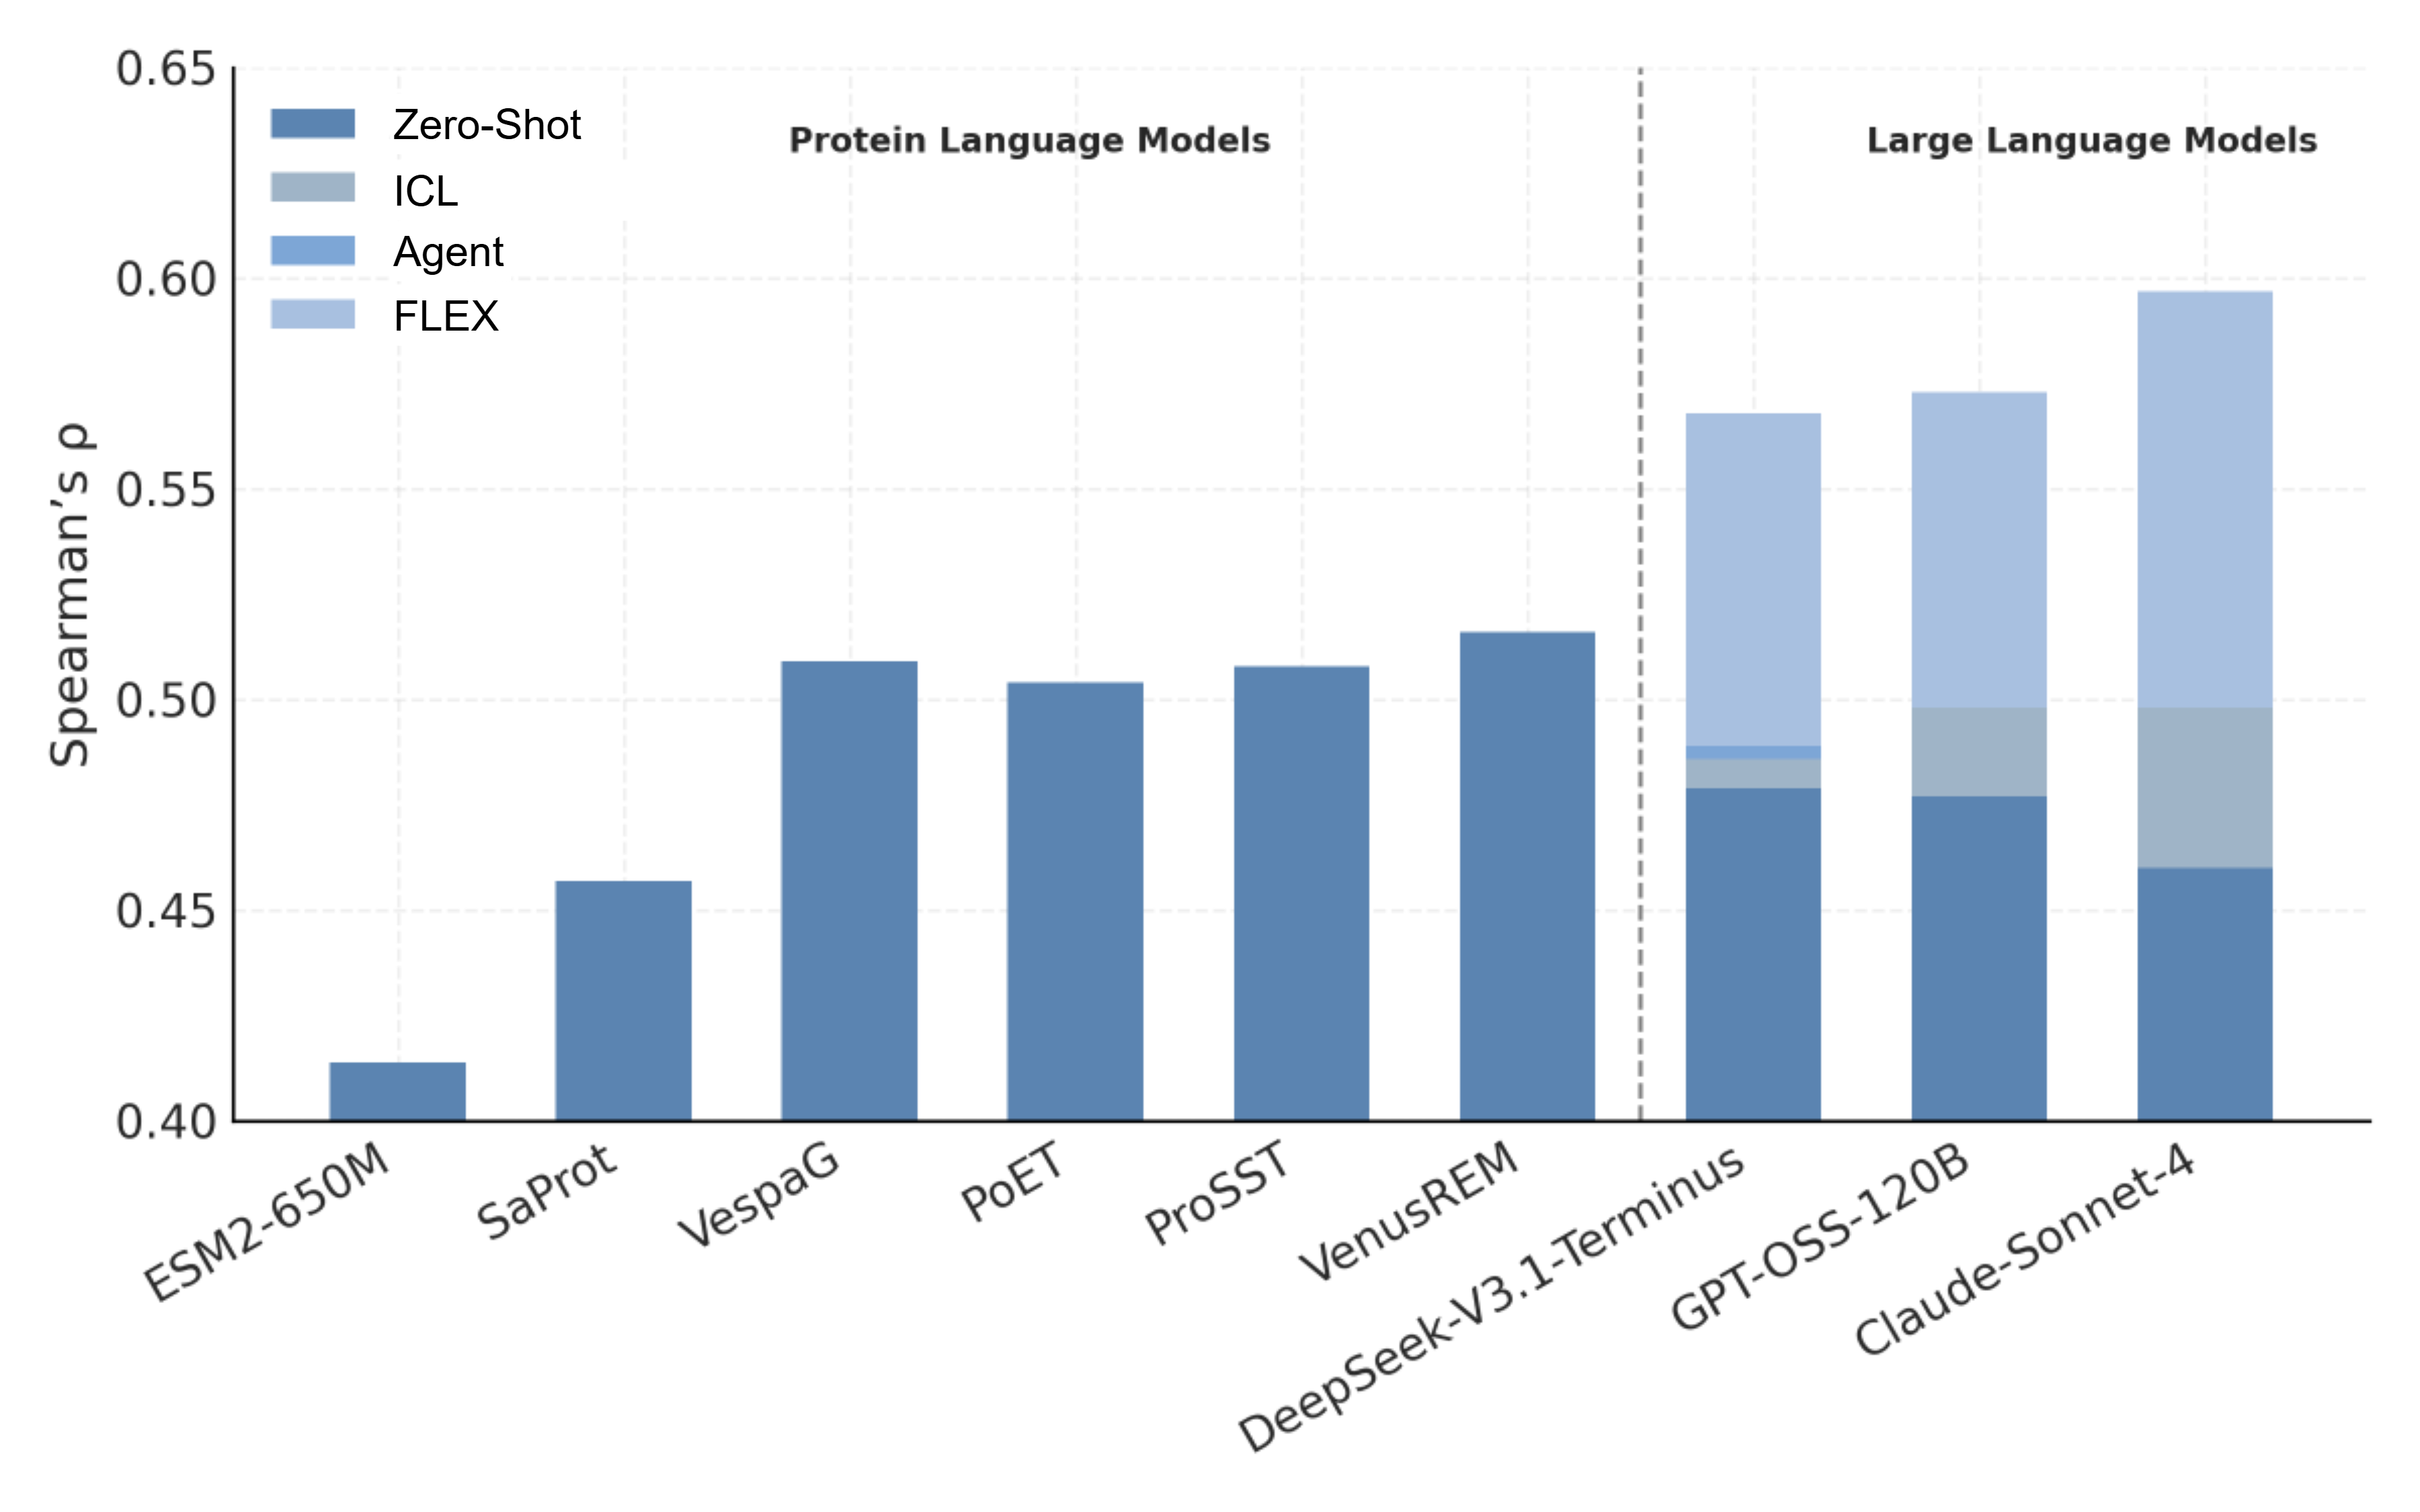
\includegraphics[width=0.98\linewidth]{./figs/proteingym_all.png}
%   \caption{ProteinGym Results from both protein language model and large language model.}
%   \label{fig:proteingym_all}
% \end{figure}

% 最后一句需要修改一下，大概意思是"不止有parameter-based training的方法可以提升模型的推理能力，我们证明了parameter-free 的方法也可以大幅提升推理能力"
\paragraph{Math.} As shown in Table~\ref{tab:main_table} and Figure~\ref{fig:main_method_overview}, our \method{} paradigm consistently and significantly outperforms all baselines across both mathematical reasoning benchmarks. On the challenging AIME25 dataset, \method{} boosts the accuracy of Claude-Sonnet-4 from a $40.0\%$ baseline to an impressive $63.3\%$ after learning from only 49 examples. This substantial $58.7\%$ relative improvement demonstrates its powerful learning capability. Similarly, on GSM8k, \method{} consistently enhances the performance of already strong models, such as elevating GPT-4's accuracy to $95.9\%$. These results demonstrate that our parameter-free paradigm can yield substantial gains in reasoning, an advancement previously achieved primarily through parameter-based learning methods~\cite{deepseekai2025deepseekr1incentivizingreasoningcapability,yu2025dapoopensourcellmreinforcement}.

\paragraph{Chemistry.} In the specialized domain of chemistry, \method{} proves to be highly effective at bridging the performance gap of generalist models. On the USPTO50k benchmark, baseline models exhibit limited proficiency, with GPT-5 and Gemini-2.5-Pro achieving only $9.0\%$ accuracy. By learning from a small set of 50 examples, \method{} nearly doubles these scores, increasing them to $16.0\% (+7.0\%)$ and $18.0\% (+9.0\%)$, respectively. The most notable gain is observed with Claude-Sonnet-4.5, which improves from $20.0\%$ to $30.0\%$ accuracy (+$10.0\%$). These results underscore the efficacy of \method{} as a sample-efficient, parameter-free approach for adapting models to complex scientific domains.


\paragraph{Biology.} For the ProteinGym zero-shot benchmark, the prevailing state-of-the-art Spearman’s correlation remains near 0.52. As shown in Table~\ref{tab:main_table} and Figure~\ref{fig:proteingym_all}, off-the-shelf large language models (LLMs) tend to underperform relative to specialized protein language models even conducting subtask of identifying and appropriately combining functionally important positions. This shortfall persists even when LLMs are supplemented with simple in-context examples, which suggests that mere exposure to a few labeled instances is insufficient to endow these models with the inductive biases required for robust mutational effect prediction. Importantly, we find that a forward-learning paradigm substantially mitigates this limitation. By extracting compact, generalizable “experience” from a small training set and encoding it as reusable rules or heuristics, the forward-learned model is able to transfer these insights to a much larger and more diverse test set — yielding an average improvement of roughly 0.10 in Spearman’s $\rho$. 







%\paragraph{The Value of Distilled Experience.} We conducted an ablation study to isolate the contribution of the experience library by comparing the standard ReAct agent to our full \method{} implementation. On AIME25, the ReAct framework alone achieves a 50.0\% accuracy, a 10.0\% absolute improvement over the naive LLM, highlighting the inherent benefit of the agentic workflow. However, \method{} extends this gain significantly, outperforming the ReAct baseline by a further 13.3\% in absolute terms (a 26.6\% relative improvement). More strikingly, an additional experiment detailed in Table~\ref{tab:main_table} shows that even when trained on the 49 problems without access to their ground-truth answers, our method still reaches 56.6\% accuracy. This result, which surpasses the standard ReAct agent by 5.6\%, underscores a critical finding: the distilled experience contains supervisory signals that are richer and potentially more valuable than ground-truth answers alone.



%\subsection{Co-evolution of Reasoning Accuracy and Experience Library.}%Training Dynamics}
\subsection{The Scaling Law of Experience}

\begin{figure}[!t]
  \centering
  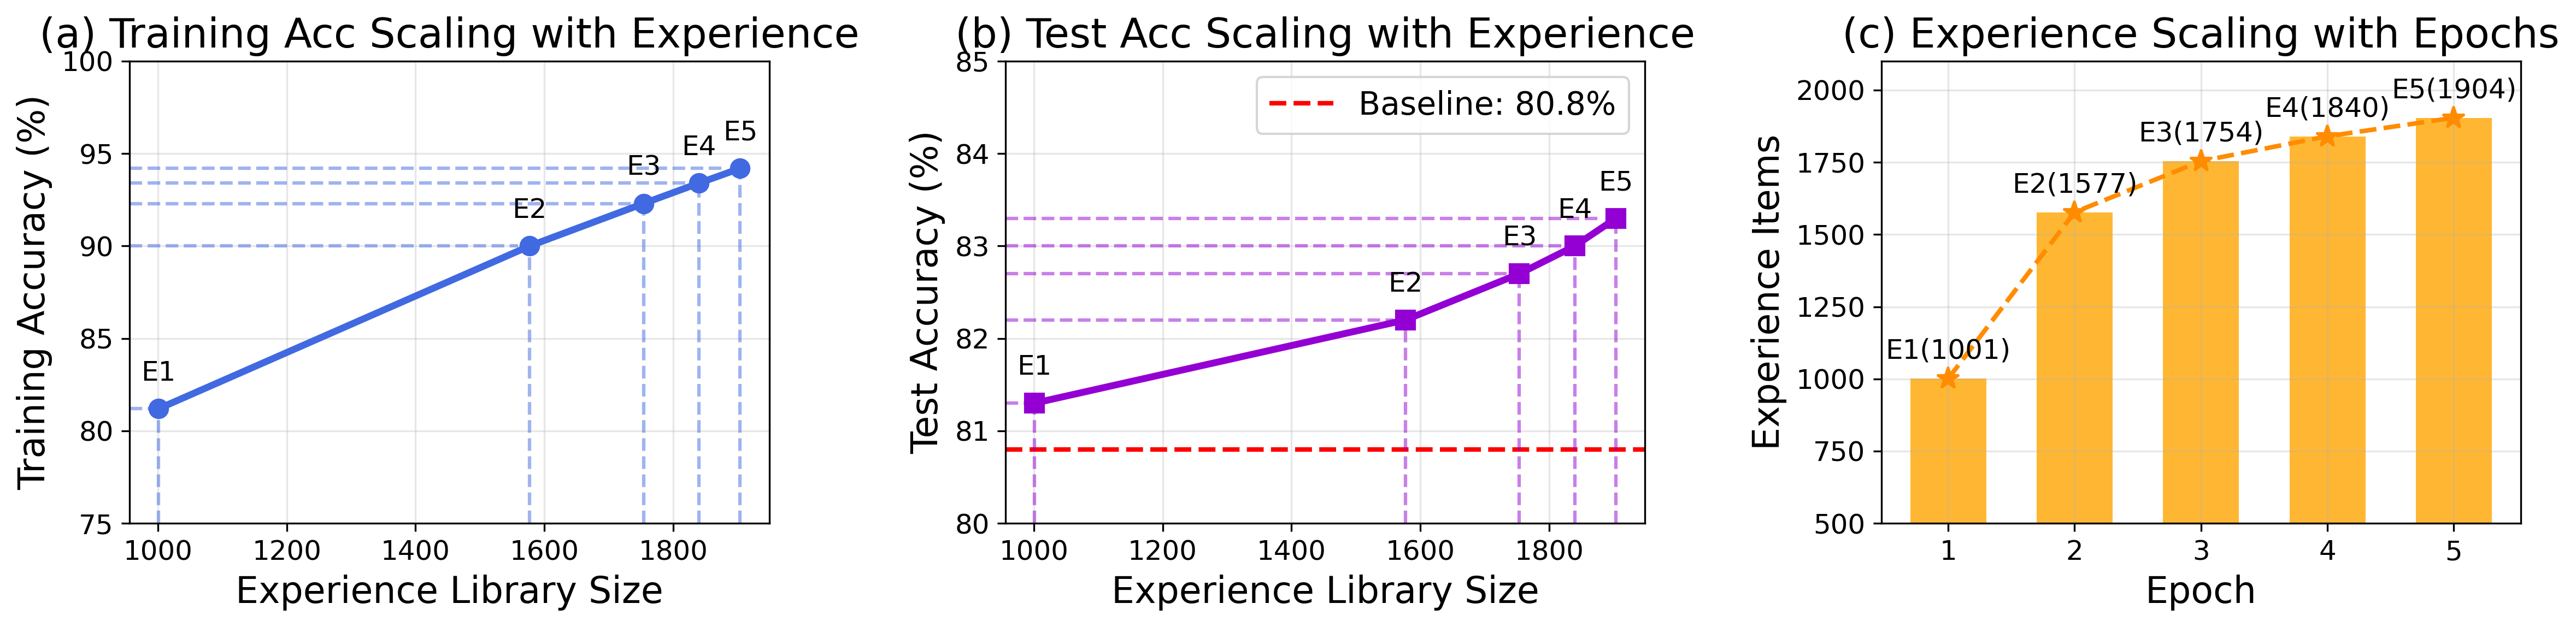
\includegraphics[width=0.98\linewidth]{./figs/scaling_law.png}
  \caption{Training dynamics and scaling laws of \method{} on the GSM8K dataset across 5 epochs. Training accuracy and test accuracy both show strong scalability with the size of the experience library. Experience library also exhibits scaling law with the epochs.}
  \label{fig:td}
\end{figure}

To understand how experience accumulation influences model performance, we systematically analyze the scaling properties of \method{}. Our investigation reveals a predictable and principled relationship between the size of the experience library and model capability. As illustrated in Fig.~\ref{fig:td}, we identify three distinct scaling regimes through rigorous analysis across 5 training epochs on GSM8k.

\textbf{Training Accuracy Scaling with Experience.} Figure~\ref{fig:td}(a) shows a strong power-law relationship, with training accuracy increasing from 81.2\% to 94.2\% as the experience library grows from 1,001 to 1,904 items. This demonstrates substantial returns from experience accumulation, with performance gains following a predictable scaling trajectory.

\textbf{Generalization Scaling with Experience.} The test accuracy in Figure~\ref{fig:td}(b) exhibits consistent improvement from 81.3\% to 83.3\%, significantly surpassing the 80.8\% baseline. The reduced variance with increasing experience indicates that accumulated knowledge stabilizes predictions and enhances reasoning robustness.

\textbf{Experience Scaling with Epochs.} Figure~\ref{fig:td}(c) uncovers a distinct scaling regime for experience accumulation itself. The process follows a logistic-like curve: rapid initial expansion (+576 experiences from epoch 1 to 2) transitions to selective refinement (+64 from epoch 4 to 5). This indicates an intelligent, phase-changing scaling law that efficiently covers the problem space while strategically avoiding redundancy.

These scaling laws establish \method{} as a principled framework for continuous model improvement, offering predictable performance gains through experience accumulation. The consistent scaling relationships across training and generalization metrics provide strong empirical grounding for experience-driven learning paradigms, suggesting new pathways for model enhancement that transcend traditional scaling approaches based solely on parameter count or compute budget to the \textbf{scaling with experience}.

\subsection{Inheritance of the Experience Library}
\begin{table}[!t]
\centering
\caption{Performance comparison on cross-model memory transfer across two benchmarks (AIME25 and USPTO50k). Values in parentheses denote the absolute accuracy improvement over the ReAct baseline for each model. The models in columns represent the source of inherited experience. For AIME25, Claude and DeepSeek in columns stand for Claude-Sonnet-4 and DeepSeek-V3.1-Teminus. For USPTO50k, GPT, Gemini, and Claude in columns stand for GPT-5, Gemini-2.5-Pro, and Claude-Sonnet-4.5. For ProteinGym, Qwen and DeepSeek in columns stand for Qwen3-8B and DeepSeek-V3.1-Terminus.}
\label{tab:memory_transfer}
\smallskip
%\renewcommand{\arraystretch}{1.2} % 行距美化，可选
%用 resizebox 强制表格宽度 = 当前 linewidth
% \resizebox{0.75\linewidth}{!}{%
\begin{tabular}{@{}lcccc@{}}
\toprule
% ======= AIME25 =======
\multicolumn{5}{c}{\textbf{AIME25}} \\
\midrule
\textbf{Model} & \textbf{Agent} & \multicolumn{2}{c}{\textbf{+ Claude}} & \textbf{+ DeepSeek} \\
\midrule
\textit{Claude-Sonnet-4} & 50.0 & \multicolumn{2}{c}{63.3 (\textcolor{blue!80}{+13.3})}  & 66.7 (\textcolor{blue!80}{+16.7}) \\
\textit{DeepSeek-V3.1-Terminus}  & 60.0  & \multicolumn{2}{c}{66.7 (\textcolor{blue!80}{+6.7})}  & 66.7 (\textcolor{blue!80}{+6.7}) \\
\midrule
% % ======= USPTO50k =======
\multicolumn{5}{c}{\textbf{USPTO50k}} \\
\midrule
 {\textbf{Model}} &  \textbf{Agent} &  {\textbf{+ GPT}} & {\textbf{+ Gemini}} &  {\textbf{+ Claude}} \\
\midrule
 {\textit{GPT-5}} &  {12.0} &  {16.0 (\textcolor{blue!80}{+4.0)} } &  18.0 (\textcolor{blue!80}{+6.0}) &  {15.0 (\textcolor{blue!80}{+3.0)} }\\
 {\textit{Gemini-2.5-Pro} } &  {12.0} &  {14.0 (\textcolor{blue!80}{+2.0)} } &  18.0 (\textcolor{blue!80}{+6.0})&  {23.0 (\textcolor{blue!80}{+11.0)} }\\
 {\textit{Claude-Sonnet-4.5} } &  {23.0} &  {28.0 (\textcolor{blue!80}{+5.0)} } &  30.0 (\textcolor{blue!80}{+7.0}) &  30.0 (\textcolor{blue!80}{+7.0)} \\
\midrule
 % ======= ProteinGym =======
\multicolumn{5}{c}{\textbf{ProteinGym}} \\
\midrule
\textbf{Model} & \textbf{Agent}& \multicolumn{2}{c}{\textbf{+ Qwen}} & \textbf{+ DeepSeek\quad\  }\\
\midrule
\textit{GPT-OSS} & {51.5} & \multicolumn{2}{c}{55.0 (\textcolor{blue!80}{+3.5})}  & 56.6 (\textcolor{blue!80}{+5.1})\\
\toprule
\end{tabular}%
% } % <-- 结束 resizebox
\end{table}




%transferability
A key advantage of \method{} over parameter-based approaches is its exceptional inheritance property (Fig~\ref{fig:inheritance}). By decoupling learned knowledge from model weights, the experience library acts as a lightweight, plug-and-play module that can be seamlessly transferred across different agents. Our experiments in Table~\ref{tab:memory_transfer} reveal two significant and economically valuable properties: the \textbf{distillation} of expertise from strong to weaker models, and the \textbf{generality} of strategies from weaker to stronger models.

First, we observe a powerful distillation effect, where expertise from a top-performing model can significantly uplift weaker ones. For instance, on USPTO50k, the experience library generated by the strongest model, Claude-Sonnet-4.5, boosts the performance of Gemini-2.5-Pro by an impressive 11 absolute points. This highlights a cost-effective pathway: the expensive exploration of a single, powerful agent can be captured and reused to enhance a fleet of less capable models without the need for individual fine-tuning. A similar trend is evident on AIME25, where the experience from the more capable DeepSeek-V3.1-Terminus model provides the largest performance gain (+16.7\%) for Claude-Sonnet-4.

Even more strikingly, our results demonstrate a strong generality effect, where experience from weaker models provides substantial benefits to stronger ones. Notably, on AIME25, the experience library from the weaker Claude-Sonnet-4 elevates the stronger DeepSeek-V3.1-Terminus by 6.7 points, achieving the exact same performance level as when DeepSeek uses its own meticulously generated experience. This finding is profound: it proves that the learned experience captures fundamental, high-level strategies that are model-agnostic, rather than model-specific artifacts. The same trend is corroborated on USPTO50k and ProteinGym, where experiences from weaker models(Qwen3-8B, DeepSeek-V3.1-Terminus, GPT-5, Gemini-2.5-Pro) substantially improve the already capable Claude-Sonnet-4.5 or GPT-OSS-120B.



Taken together, these phenomena establish the experience library as a truly portable knowledge module. This opens a path towards a new paradigm: creating a single, universal experience library through a one-time training process, or even mixing experiences from diverse sources, to provide general performance improvements across a wide ecosystem of agents.

\begin{figure}[!htbp]
    \centering
    
\includegraphics[width=0.8\linewidth]{figs/case_study.png}
    \caption{Qualitative case studies in Mathematics, Chemistry, and Biology demonstrating the effectiveness of \method{}. In each domain, baseline agents (LLM Response, ReAct Response) fail due to critical reasoning errors (marked with \textcolor{red}{\ding{55}}). In contrast, by retrieving and applying distilled knowledge (\textit{e.g.}, Golden rules and Warnings) from its experience library, \method{} successfully refines its strategy, overcomes the initial failures, and arrives at the correct solution (marked with \textcolor{green!70!black}{\ding{51}}).}
    \label{fig:case_study}
\end{figure}

\subsection{Case Study}
This section presents case studies across three domains to illustrate how the learned experience library by \method{} corrects initial failures by providing critical procedural knowledge and transforms flawed reasoning into correct solutions.

\paragraph{Math.} The distinct problem-solving trajectories in Figure~\ref{fig:case_study} highlight the transformative impact of our \method{} paradigm. The naive LLM fails by decoupling geometric constraints, leading to infeasible side lengths. The standard ReAct agent, while more structured, drifts into special-case assumptions without verifying global consistency. In stark contrast, \method{} leverages its experience library to inject structured, procedural knowledge into the reasoning cycle. By retrieving a reusable algebraic template and critical feasibility checks (e.g., $a^2 + b^2 = 1444$, $a,b \le 28$), it directly addresses the core LLM limitations of logical drift and constraint violation. This distilled experience transforms the agent's process from a heuristic-driven exploration into a deterministic, solve-verify loop, pruning invalid branches and enforcing global reconciliation. Essentially, the experience library provides the procedural scaffolds and logical guardrails that the other approaches lack, enabling the agent to systematically find the correct parameters and compute the final area of $104\sqrt{3}$. This demonstrates how our paradigm bridges the gap between an LLM's declarative knowledge and the effective procedural execution required for complex problem-solving.

\paragraph{Chemistry.} The trajectories in Figure~\ref{fig:case_study} reveal a critical gap in the domain-specific reasoning of standard models. Both the naive LLM and the vanilla ReAct agent make the same fundamental error: despite correctly identifying the mesylate group, they misidentify the disconnection point by prioritizing a plausible but incorrect N-alkylation pathway. This demonstrates a failure to translate declarative knowledge (what a mesylate is) into correct procedural execution (how to disconnect it). In stark contrast, \method{} succeeds by leveraging its experience library to bridge this gap. It retrieves an explicit template ($\mathrm{R{-}O{-}SO_2{-}CH_3} \rightarrow \mathrm{R{-}OH} + \mathrm{CS(=O)(=O)Cl}$) that overrides the flawed heuristic and enforces the canonical $\mathrm{O{-}S}$ bond disconnection. The experience library thus functions as an external knowledge substrate, injecting proven procedural scaffolds and domain-specific constraints into the agent's workflow. This transforms the reasoning process from speculative hypothesis testing into a deterministic, domain-grounded execution, ensuring the correct retrosynthesis is identified.

\paragraph{Biology.} Figure~\ref{fig:case_study} provides an example of how agents learn from a deliberately designed experience library—golden rules, warnings, and core know-how. Unlike the math and retro-synthesis problems above, protein-fitness prediction rarely admits absolute right/wrong answers; instead, useful guidance must be distilled from empirical trial trajectories and cross validation signals. The library captures those trajectories as reusable micro-strategies and failure patterns, enabling the agent to adapt a generic regression objective to the idiosyncrasies of a specific protein. In practice this means shifting attention away from globally renowned, aggregate metrics toward complementary, target-specific features and modeling choices that actually improve performance on the individual proteins. Moreover, the distilled tips actively drive algorithmic evolution: they suggest pre-processing pipelines, more detailed feature-combination heuristics, and validation gates that make final formula more robust. By overlaying proven procedural scaffolds onto the frozen LLM’s answer, the experience library encourages more valuable and diverse explorations and simultaneously enlarges meaningful solutions that better tuned to the peculiarities scenarios.